

\documentclass[14pt,a4paper]{extreport}

\usepackage[utf8]{inputenc}
\usepackage[T2A]{fontenc}

\usepackage{tempora}

\usepackage[english,russian]{babel}

\usepackage{amsmath,amssymb,amsfonts}
\usepackage{graphicx}
\usepackage{geometry}
\usepackage{float}
\usepackage{caption}
\usepackage{subcaption}
\usepackage{booktabs}
\usepackage{multirow}
\usepackage{listings}
\usepackage{xcolor}
\usepackage{setspace}
\usepackage{titlesec}
\usepackage{fancyhdr}
\usepackage{tocloft}
\usepackage{cite}
\usepackage{hyperref}

\geometry{left=30mm,right=15mm,top=20mm,bottom=20mm}

\onehalfspacing

\setlength{\parindent}{1.25cm}
\setlength{\parskip}{0pt}

\titleformat{\chapter}[block]
  {\centering\fontsize{16pt}{20pt}\selectfont\bfseries}
  {Глава \thechapter.}{0.5em}{}
\titleformat{name=\chapter,numberless}[block]
  {\centering\fontsize{16pt}{20pt}\selectfont\bfseries}
  {}{0pt}{}
\titlespacing*{\chapter}{0pt}{0pt}{1.5em}

\titleformat{\section}[block]
  {\centering\fontsize{14pt}{18pt}\selectfont\bfseries}
  {\thesection.}{0.5em}{}
\titlespacing*{\section}{0pt}{1.2em}{0.8em}

\titleformat{\subsection}[block]
  {\centering\fontsize{14pt}{18pt}\selectfont\bfseries}
  {\thesubsection.}{0.5em}{}
\titlespacing*{\subsection}{0pt}{1em}{0.6em}

\pagestyle{fancy}
\fancyhf{}
\fancyfoot[C]{\thepage}
\renewcommand{\headrulewidth}{0pt}
\renewcommand{\footrulewidth}{0pt}

\fancypagestyle{plain}{
  \fancyhf{}
  \fancyfoot[C]{\thepage}
  \renewcommand{\headrulewidth}{0pt}
  \renewcommand{\footrulewidth}{0pt}
}

\renewcommand{\cftchapfont}{\bfseries}
\renewcommand{\cftchappagefont}{\bfseries}

\hypersetup{
    colorlinks=true,
    linkcolor=black,
    citecolor=black,
    urlcolor=blue
}

\lstset{
    basicstyle=\ttfamily\footnotesize,
    breaklines=true,
    frame=single,
    language=Python,
    keywordstyle=\color{blue},
    commentstyle=\color{gray},
    showstringspaces=false,
}

\title{
    \textbf{Классификация клеток в цитоскрининге\\
    с использованием гибридной архитектуры\\
    Vision Transformer и сверточных нейронных сетей}\\[1em]
    \large Выпускная квалификационная работа\\
    Направление: Искусственный Интеллект и Компьютерное Зрение
}
\author{А.~О.~Маскаев}
\date{Нижний Новгород, \the\year}

\begin{document}

\maketitle
\thispagestyle{empty}
\setcounter{page}{2}

\begin{abstract}
Рак шейки матки является четвёртой по частоте причиной заболеваемости и
смертности от рака среди женщин в мире. Ранняя диагностика с помощью
цитологического скрининга мазков Папаниколау позволяет существенно повысить
выживаемость пациентов. В данной работе представлена гибридная модель для
многоклассовой классификации клеток в цитоскрининге, объединяющая
сверточную нейронную сеть ConvNeXt и кодировщик Vision Transformer.
Модель обучена на датасете SIPaKMeD, содержащем 4\,049 изображений
изолированных клеток (подмножество CROPPED) пяти классов. В отличие от предыдущих работ, применяется стратифицированное
разбиение на обучающую/валидационную/тестовую выборки, обеспечивающее
сбалансированное представление классов. Обучение выполнено с использованием
label smoothing, Mixup-аугментации, RandAugment, stochastic depth и
раздельных learning rate для backbone и трансформерной части.
Эксперименты на отложенной тестовой выборке демонстрируют Accuracy 95.51\%,
F1-score (macro) 95.48\% и AUC-ROC (macro) 99.72\%. Аблационное сравнение
с базовой моделью без трансформерной части подтверждает вклад каждого
компонента архитектуры. По итогам работы подготовлены: воспроизводимый
программный пакет с интерфейсом командной строки, набор обученных
контрольных точек модели, скрипты построения графиков обучения и
матриц ошибок, а также модуль визуализации attention rollout для
интерпретации решений модели.

\textbf{Ключевые слова:} рак шейки матки, цитология, мазок Папаниколау,
компьютерное зрение, Vision Transformer, ConvNeXt, стохастическая глубина,
Mixup, классификация изображений.
\end{abstract}


\renewcommand{\contentsname}{Оглавление}
\tableofcontents
\clearpage

\chapter*{Введение}
\addcontentsline{toc}{chapter}{Введение}
\label{ch:intro}

Рак шейки матки остаётся одной из ключевых проблем онкологической
помощи женщинам. По данным GLOBOCAN, ежегодно в мире регистрируется более
600\,000 новых случаев заболевания и около 340\,000 летальных исходов
\cite{bray2018global}. При этом раннее выявление предраковых изменений
позволяет добиться пятилетней выживаемости более 90\% \cite{curry2018screening}.
Распределение заболеваемости неоднородно: в странах с развитыми скрининговыми
программами смертность от рака шейки матки за последние десятилетия снизилась в разы, тогда
как в регионах с ограниченным доступом к цитологическому обследованию остаётся
высокой. Эта неравномерность связана не столько с биологией заболевания,
сколько с организационными и кадровыми факторами.

Цитологический скрининговый тест по Папаниколау (Pap test), предложенный
Г.~Папаниколау в 1928 г. и распространившийся в клинической практике с
1940-х годов, и его модификации на основе жидкостной цитологии (LBC) являются
основными методами ранней диагностики \cite{hashmi2020comparison}.
Стандартная процедура предполагает забор клеточного материала с поверхности
шейки матки, фиксацию на стекле, окрашивание по Папаниколау и последующий
визуальный анализ препарата врачом-цитологом. Несмотря на длительную историю
и относительную простоту метода, в нём заложено два фундаментальных
ограничения. Первое - субъективность интерпретации: согласованность
заключений двух независимых цитологов на неоднозначных, пограничных
препаратах остаётся умеренной. Количественно это выражается коэффициентом
каппа Коэна, который для таких случаев редко превышает 0.6 по шкале от 0
(совпадение на уровне случайного угадывания) до 1 (полное совпадение
заключений); порогом клинической надёжности обычно считается значение не
ниже 0.8 \cite{branca2015recommendations}. Второе ограничение - высокая
трудоёмкость: один скрининг-препарат содержит десятки тысяч клеток, из
которых патологически изменены могут быть единичные. К концу рабочего дня
усталость цитолога закономерно ведёт к росту числа ложноотрицательных
заключений.

Идея автоматизировать поиск аномальных клеток на цитологическом препарате не
нова. Первые коммерческие системы CAD - PAPNET (1990-е годы) - использовали
многоуровневый нейросетевой каскад для отбора подозрительных клеток с
последующей ручной верификацией. Распространения они не получили
прежде всего из-за низкой точности и высокой стоимости. С появлением
свёрточных нейронных сетей (CNN) в 2010-х годах и их доминирования в задачах
компьютерного зрения \cite{lecun2015deep} интерес к автоматизированной
цитологии возобновился. Архитектуры ResNet, EfficientNet и более новые
семейства способны извлекать локальные текстурные и морфологические
признаки клетки с точностью, недостижимой для классических методов
ручной разметки признаков.

Параллельно с CNN в области компьютерного зрения возник альтернативный
подход - Vision Transformer (ViT). Идея заключается в обработке изображения
как последовательности фиксированных patch-токенов с применением механизма
self-attention, заимствованного из обработки естественного языка. ViT не
имеет встроенной трансляционной инвариантности и иерархического спуска,
характерных для CNN, но взамен моделирует попарные зависимости между
произвольно удалёнными участками изображения. Для медицинских данных это
свойство потенциально ценно: например, для классификации клетки важна
\textit{совокупная} оценка соотношения ядро/цитоплазма и характеристик
околоядерного гало, то есть глобальный контекст внутри клетки. На практике
чистый ViT требует большого объёма обучающих данных, что плохо согласуется
с типичными размерами медицинских датасетов. Поэтому в последние годы
развивалось семейство \textit{гибридных} архитектур CNN+ViT, в
которых CNN-стадия извлекает локальные признаки, а трансформер агрегирует
глобальный контекст по карте признаков.

В цитологии эти архитектуры начали применяться буквально в последние годы.
В работах \cite{cerviformer2023, cervigan2025, hybridvit2025} приводятся
впечатляющие цифры точности на SIPaKMeD - 96--99\%. Однако в большинстве
публикаций отсутствует явное обсуждение того, как именно выполнялся сплит
датасета. SIPaKMeD структурно содержит несколько клеток, вырезанных с
одного и того же исходного слайда; если случайное разбиение не учитывает
эту группировку, клетки одного слайда оказываются одновременно и в
обучающей, и в тестовой выборках. Тогда модель может запомнить специфичные
для конкретного слайда артефакты - оттенок окраски конкретной партии
красителя, особенности освещения и калибровки микроскопа, анатомические
особенности тканей данной пациентки - и выдать высокую тестовую точность,
опираясь на эти признаки вместо общих цитологических. В реальном применении
такая модель сталкивается с препаратами совершенно новых пациентов, на
которых эти подсказки отсутствуют, и точность резко падает. Поэтому в
медицинской задаче честная оценка должна моделировать именно обобщение на
\textit{нового пациента}, а не на новую клетку уже известного. Случайное
разбиение без группировки систематически завышает заявляемые в литературе
проценты и затрудняет сопоставление методов между собой.

Настоящая работа отталкивается от этих наблюдений. Помимо построения
гибридной CNN+ViT модели, в ней последовательно реализуется ряд методических
требований: явная группировка по слайду в стратифицированном сплите,
полный воспроизводимый пайплайн, аблационное сравнение с baseline-моделью
без трансформера и кросс-валидация для количественной оценки дисперсии.
Дополнительно реализована визуализация attention rollout, позволяющая
проверить, что модель основывает решение на биологически значимых регионах
клетки.

\textbf{Цель работы} - разработать продвинутую модель многоклассовой
классификации клеток в цитоскрининге на основе гибридной архитектуры CNN +
Vision Transformer и провести её оценку на публичном датасете SIPaKMeD с
методически корректной процедурой валидации, включающей: (1)
стратифицированное разбиение с группировкой по слайду
(\texttt{StratifiedGroupKFold}) для исключения утечки признаков пациента
между обучающей и тестовой выборками; (2) пятикратную кросс-валидацию
с отчётом среднего и стандартного отклонения метрик; (3) использование
отложенной тестовой выборки, не задействованной при подборе
гиперпараметров.

\textbf{Задачи работы:}
\begin{enumerate}
    \item Провести анализ современных методов автоматизированного анализа
          цитологических изображений.
    \item Реализовать корректный пайплайн загрузки данных SIPaKMeD с
          верификацией полноты выборки и стратифицированным разбиением.
    \item Реализовать гибридную модель (ConvNeXt + Transformer encoder)
          с усовершенствованными техниками регуляризации и обучения.
    \item Провести эксперименты на датасете SIPaKMeD и сравнить результаты
          с базовыми подходами из литературы.
    \item Оформить программную реализацию в воспроизводимый пакет.
\end{enumerate}

\textbf{Научная новизна} заключается в применении расширенного набора техник
(stochastic depth, label smoothing, Mixup, RandAugment, раздельные LR) к
гибридной CNN-Transformer архитектуре на датасете SIPaKMeD, а также в
выявлении и исправлении типичной ошибки пайплайна загрузки данных, приводящей
к нулевой обучающей выборке при вложенной структуре директорий.

\textbf{Практическая значимость} - разработанная модель может использоваться
как компонент системы компьютерной помощи цитологу (CAD) при скрининге рака
шейки матки.

\chapter{Обзор литературы и постановка задачи}
\label{ch:literature}

\section{Цитологический скрининг и классификация клеток}

Стандартом классификации результатов Pap-теста является система Bethesda
(TBS), последняя редакция которой относится к 2014 году. TBS вводит
терминологию, объединяющую цитологические и гистологические находки в единую
шкалу степеней дисплазии: NILM (отсутствие интраэпителиальных поражений),
ASC-US, ASC-H, LSIL, HSIL, AGC, и карцинома. На уровне отдельной клетки эта
классификация опирается на ряд морфологических признаков: размер и форма ядра,
ядерно-цитоплазматическое соотношение (N/C ratio), гипохромия ядра, наличие
перинуклеарного гало, многоядерность, неровность контура ядра
\cite{randel2013acog}. Опытный цитолог распознаёт эти признаки за доли
секунды, но формализация их в виде воспроизводимых количественных правил
оказывается нетривиальной.

Датасет SIPaKMeD \cite{plissiti2018sipakmed}, использованный в настоящей
работе, организует клетки в пять цитологических классов:
\begin{itemize}
    \item \textbf{Superficial-Intermediate} - нормальные плоские клетки
          поверхностного и промежуточного слоёв многослойного эпителия.
          Крупные, с малым ядерно-цитоплазматическим соотношением, обильной
          эозинофильной или базофильной цитоплазмой. Преобладают в препарате
          здоровой женщины репродуктивного возраста.
    \item \textbf{Parabasal} - нормальные клетки базального слоя, мелкие,
          с относительно крупным ядром. В мазке здоровой женщины
          репродуктивного возраста встречаются редко, но их доля растёт в
          постменопаузальный период за счёт атрофических изменений эпителия;
          в этом возрастном контексте они считаются нормой.
    \item \textbf{Koilocytotic} - клетки с койлоцитозом: перинуклеарным
          гало («ореолом») вокруг сморщенного гиперхромного ядра. Это
          ключевой цитопатический признак инфекции вирусом папилломы
          человека (ВПЧ), включая онкогенные типы.
    \item \textbf{Dyskeratotic} - ороговевающие клетки с уплотнённой
          цитоплазмой и пикнотическим ядром. Их присутствие в значительном
          количестве типично для плоскоклеточных интраэпителиальных
          поражений и плоскоклеточной карциномы.
    \item \textbf{Metaplastic} - доброкачественные метапластические клетки,
          возникающие в зоне трансформации (стык плоского и
          цилиндрического эпителия). Считаются нормальной реакцией ткани,
          но морфологически сходны с диспластическими клетками - именно
          из них при дальнейшем прогрессе возникает плоскоклеточная
          неоплазия.
\end{itemize}

Из пяти классов SIPaKMeD три (Superficial-Intermediate, Parabasal,
Metaplastic) клинически рассматриваются как нормальные или
доброкачественные, а два (Koilocytotic, Dyskeratotic) - как однозначно
аномальные. С точки зрения автоматизированного скрининга минимальной
рабочей задачей было бы бинарное разделение норма/аномалия. Однако
многоклассовая постановка сохраняет диагностическую интерпретируемость
выхода модели: койлоцитоз и дискератоз указывают на разные клинические
сценарии (ВПЧ-инфекция vs дисплазия) и ведут к разным протоколам
дальнейшего обследования. Поэтому в литературе и в данной работе
рассматривается именно пятиклассовая задача.

\section{Развитие нейросетевых архитектур для зрения}

Кратко обозначим линию архитектурных идей, релевантных для
рассматриваемой задачи, поскольку их понимание необходимо для обоснования
выбора в \S\ref{ch:methodology}.

CNN-эра в компьютерном зрении задана работами LeCun et al. (LeNet, 1998),
Krizhevsky et al. (AlexNet, 2012), He et al. (ResNet, 2015) - каждая
следующая архитектура решала проблему предыдущей за счёт остаточных
связей, batch-нормализации, увеличения глубины. Семейство EfficientNet
(Tan and Le, 2019) формализовало масштабирование по глубине, ширине и
разрешению; этот подход остаётся одним из стандартов для медицинского
зрения.

Появление Vision Transformer \cite{liu2022convnext}\footnote{В качестве
основной работы по ViT часто цитируется Dosovitskiy et al. ICLR 2021;
здесь мы ссылаемся на работу ConvNeXt, в которой проводится подробное
сравнение CNN и ViT.} разделило сообщество. ViT режет изображение на
непересекающиеся патчи $16 \times 16$ или $32 \times 32$, кодирует их
линейной проекцией и обрабатывает стандартным трансформерным энкодером.
Self-attention позволяет каждому patch-токену в каждом слое получать
информацию от всех остальных - глобальная связность с первого слоя.
У этого подхода два недостатка: квадратичная сложность по числу токенов
и отсутствие индуктивных приоров (трансляционная инвариантность,
локальность), что требует существенно больших данных для обучения.

Ответом со стороны CNN-семейства стал ConvNeXt \cite{liu2022convnext}.
Авторы постадийно модернизировали ResNet, перенимая инсайты из ViT:
большие depth-wise свёртки $7 \times 7$, инвертированные «бутылочные»
блоки, LayerNorm вместо BatchNorm, GELU вместо ReLU. Получившаяся
архитектура сохраняет вычислительную эффективность CNN, но приближается
к ViT по точности на больших датасетах. Принципиально важно, что ConvNeXt
выдаёт пространственную карту признаков (а не один глобальный вектор),
что делает её удобным CNN-бэкбоном для гибридов с трансформерным
энкодером.

\section{Методы глубокого обучения в цитологии}

\subsection{Детекция клеток}

X.~Li и Q.~Li \cite{li2019detection} применили Faster R-CNN для детекции и
классификации цервикальных клеток на ранних версиях наборов данных
Herlev/SIPaKMeD. Xiang и др. \cite{xiang2020novel} построили двухступенчатую
схему: YOLOv3 для быстрой детекции потенциально аномальных регионов и
каскадный классификатор для уточнения класса. Ma и др. \cite{ma2020macd}
предложили MACD R-CNN на основе Mask R-CNN, рассчитанный на сегментацию
клеточных ядер с одновременной классификацией.

Zhang и др. \cite{zhang2025large} представили крупный публичный датасет
HMCHH-TCT-CellDet (8\,037 изображений ТСТ-цитологии), на котором
сравнили работу современных детекторов: Faster R-CNN, RetinaNet, YOLO
v5/v8, DETR. Авторы делают вывод, что DETR-семейство достигает
сопоставимой точности при меньшем числе ложноположительных боксов, что
важно в скрининговом контексте. Эта работа не пересекается с нашей по
задаче (мы решаем classification, а не detection), но даёт более широкий
контекст направления: детекция важна для пакетной обработки полей зрения
со слайда, тогда как классификация изолированных клеток - естественный
этап после сегментации.

\subsection{Классификация клеток}

Plissiti и др. \cite{plissiti2018sipakmed} в работе, представившей сам
датасет SIPaKMeD, использовали классический подход: извлечение 26
морфологических признаков (площадь, периметр, ядерно-цитоплазматическое
соотношение, моменты Зернике, текстурные дескрипторы Харалика) с
последующим обучением SVM и MLP. Достигнутая точность ($\approx 89$\% на
пятиклассовой задаче) демонстрировала верхнюю границу для feature-based
методов и одновременно мотивировала переход к end-to-end DL.

В последующие годы появились работы, последовательно поднимавшие точность
на SIPaKMeD за счёт более продвинутых DL-архитектур и техник аугментации.
CerviFormer \cite{cerviformer2023} применяет cross-attention между
исходным изображением и обучаемым набором латентных запросов, на основе
которых формируется итоговое представление; авторы сообщают точность
96.2\%. CerviGAN \cite{cervigan2025} использует GAN-аугментацию: GAN-сеть
обучается на исходном датасете и порождает синтетические изображения
для редких классов, после чего на расширенной выборке обучается
External-Attention-Transformer. Достигнутая точность - 98.5\%, однако
этот результат стоит интерпретировать с осторожностью: синтетические
сэмплы, полученные тем же датасетом, на котором затем оценивается модель,
способны систематически смещать оценку. Гибрид Vision Transformer с
ансамблем CNN \cite{hybridvit2025} приводит цифру 99.18\%, но при этом
сообщает использование ансамблирования из нескольких CNN-моделей и не
описывает детально процедуру сплита.

Общая особенность литературы по SIPaKMeD - слабая методическая
сравнимость результатов между статьями. В \cite{plissiti2018sipakmed}
используется одна схема разбиения, в \cite{cerviformer2023} - другая, в
\cite{hybridvit2025} - третья, причём в части работ просто отсутствует
явное описание процедуры. Поскольку SIPaKMeD содержит \textit{кропы} с
небольшого числа исходных слайдов, наивное случайное разбиение неизбежно
приводит к утечке между train и test (соседние клетки одного слайда
лежат в разных подвыборках). Игнорирование этой утечки - одна из
причин завышенных абсолютных цифр в существующих работах.

\subsection{Аугментация и регуляризация}

Параллельно с архитектурным прогрессом развивался стек техник аугментации
и регуляризации. Mixup \cite{zhang2018mixup} вводит линейную интерполяцию
между парами обучающих сэмплов и их метками, что эмпирически снижает
переобучение и улучшает калибровку. RandAugment \cite{cubuk2020randaugment}
заменяет ручной подбор аугментаций случайной выборкой из заранее
заготовленного пула с единственным параметром «магнитуды».
Stochastic depth (DropPath) \cite{huang2016deep} случайно отключает
блоки сети во время обучения, что эквивалентно неявному обучению ансамбля
сетей различной глубины. Label smoothing смягчает one-hot цели и
снижает overconfidence в предсказаниях. В современных рецептах обучения
(timm, DeiT, ConvNeXt) эти приёмы применяются \textit{одновременно}; в
данной работе используется именно такой комбинированный подход.

\section{Пробелы в литературе и место данной работы}

На основании обзора можно выделить несколько практических пробелов в
существующих работах по классификации SIPaKMeD:
\begin{enumerate}
    \item Отсутствие явной группировки по слайду при разбиении ведёт к
          утечке и завышению метрик.
    \item Большинство работ сообщают одну цифру точности по одному
          сплиту, без оценки дисперсии (нет кросс-валидации или
          доверительных интервалов).
    \item Реализационные детали (точные гиперпараметры, конфиги,
          процедура воспроизведения) часто не публикуются вместе с
          результатами.
    \item Сравнение архитектурных решений редко проводится в виде
          аблации на едином сплите: чаще каждая работа сравнивает свой
          новый метод с цифрами из других работ, полученными в иных
          условиях.
    \item Интерпретируемость решений модели (attention rollout,
          Grad-CAM) обсуждается лишь эпизодически.
\end{enumerate}

Данная работа закрывает каждый из этих пробелов хотя бы частично:
используется \texttt{StratifiedGroupKFold} с группировкой по слайду,
проводится 5-fold CV для количественной оценки $\sigma$, публикуется
исходный код в виде Python-пакета с CLI и конфигами, проводится
аблационное сравнение baseline vs hybrid на едином сплите, и реализована
визуализация attention rollout для интерпретации.

\section{Постановка задачи}

Задача формулируется как многоклассовая классификация: по входному изображению
клетки $x \in \mathbb{R}^{H \times W \times 3}$ предсказать метку класса
$y \in \{0,1,2,3,4\}$, соответствующую одному из пяти типов клеток.

Оценка производительности:
\[
    \text{Accuracy} = \frac{1}{N}\sum_{i=1}^{N}\mathbf{1}[\hat{y}_i = y_i],
    \quad
    \text{F1}_{\text{macro}} = \frac{1}{C}\sum_{c=1}^{C}
        \frac{2 \cdot \text{Pr}_c \cdot \text{Re}_c}
             {\text{Pr}_c + \text{Re}_c},
\]
где $C=5$ - число классов, $\text{Pr}_c$ и $\text{Re}_c$ - точность и
полнота по классу $c$.

\chapter{Методология}
\label{ch:methodology}

\section{Датасет SIPaKMeD}

Используется датасет SIPaKMeD \cite{plissiti2018sipakmed} в варианте
Cervical Cancer Largest Dataset (SIPaKMeD) с платформы Kaggle
\cite{kaggle_sipakmed}. В работе используется подмножество изолированных
клеток - каталог \texttt{CROPPED/}, содержащий \textbf{4\,049 изображений}
клеток в формате BMP, распределённых по пяти классам
(табл.~\ref{tab:dataset}). Дополнительные cluster-images, содержащие
несколько клеток на одном кадре, исключены из обучения, поскольку
single-label классификация для них некорректна.

\begin{table}[H]
\centering
\caption{Распределение изображений по классам в SIPaKMeD (CROPPED)}
\label{tab:dataset}
\begin{tabular}{lcc}
\toprule
Класс & Количество & Доля (\%) \\
\midrule
Superficial-Intermediate & 831  & 20.5 \\
Parabasal                & 787  & 19.4 \\
Koilocytotic             & 825  & 20.4 \\
Dyskeratotic             & 813  & 20.1 \\
Metaplastic              & 793  & 19.6 \\
\midrule
\textbf{Итого}           & \textbf{4049} & 100.0 \\
\bottomrule
\end{tabular}
\end{table}

\begin{figure}[H]
\centering
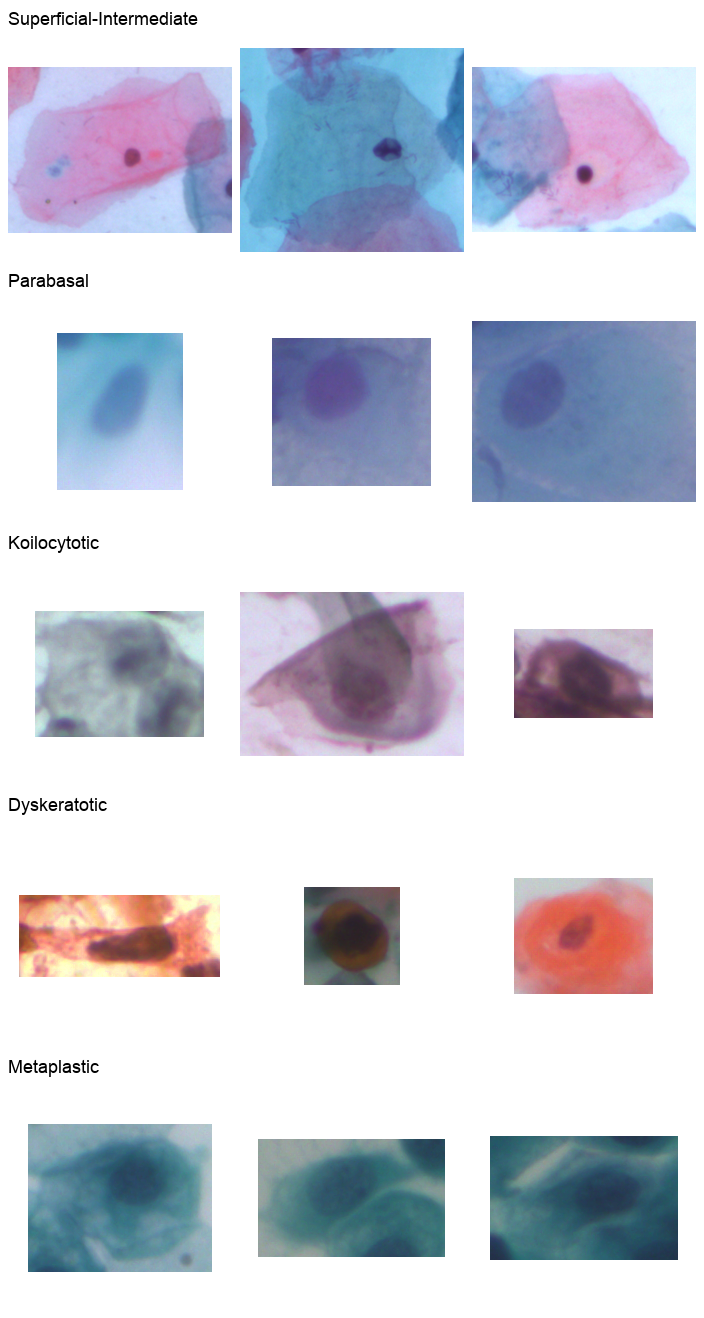
\includegraphics[width=0.95\textwidth,height=0.78\textheight,keepaspectratio]{figures/dataset_examples.png}
\caption{Примеры изолированных клеток из подмножества CROPPED датасета
SIPaKMeD: по три случайно выбранных представителя каждого из пяти
классов. Видна выраженная морфологическая вариативность внутри классов
(размер клетки, форма ядра, оттенок окрашивания) и характерные
цитопатические признаки: малое ядерно-цитоплазматическое соотношение
у Superficial-Intermediate, перинуклеарное гало у Koilocytotic,
ороговевающая цитоплазма у Dyskeratotic.}
\label{fig:dataset_examples}
\end{figure}

\subsection{Структура файлов и пайплайн загрузки}

Архив Kaggle имеет \textit{вложенную} структуру:
\begin{lstlisting}
sipakmed/
  im_Dyskeratotic/
    im_Dyskeratotic/     <- images here
      *.bmp
      CROPPED/           <- CROPPED variant (same class)
  ...
\end{lstlisting}

Изображения находятся \textit{на один уровень глубже} папки класса, а
изолированные клетки - ещё на уровень глубже, в подкаталоге
\texttt{CROPPED/}. Это является распространённой ошибкой реализации: если при
обходе файловой системы использовать \texttt{os.listdir()} или
\texttt{Path.iterdir()} без рекурсии, обучающие выборки окажутся пустыми -
модель будет обучаться на нулевых данных. В данной работе пайплайн загрузки
явно адресует подкаталог \texttt{CROPPED/} каждого класса
(см. \texttt{datasets/sipakmed.py}), что корректно находит все 4\,049
изображений изолированных клеток.

\subsection{Разбиение на выборки}

Применяется \textbf{стратифицированное} разбиение 70\%/15\%/15\%
(train/val/test) с фиксированным seed=42. Стратификация гарантирует, что
распределение классов в каждой подвыборке соответствует общему
(табл.~\ref{tab:split}).

\begin{table}[H]
\centering
\caption{Стратифицированное разбиение датасета (с группировкой по слайду)}
\label{tab:split}
\begin{tabular}{lccc}
\toprule
Подвыборка & Размер & Доля (\%) \\
\midrule
Train & 2880 & 71.1 \\
Val   & 590  & 14.6 \\
Test  & 579  & 14.3 \\
\midrule
\textbf{Итого} & \textbf{4049} & 100.0 \\
\bottomrule
\end{tabular}
\end{table}

Точные числа в подвыборках отличаются от номинальных 70/15/15, поскольку
\texttt{StratifiedGroupKFold} сохраняет целостность групп (все клетки с
одного слайда попадают в одну подвыборку), что предотвращает утечку признаков
пациента/слайда между train и test. Train также проходит через DataLoader с
\texttt{drop\_last=True} для устойчивости BatchNorm/LayerNorm на последнем
батче.

\section{Аугментация данных}
\label{sec:augmentation}

Размер обучающей выборки - около 2880 сэмплов - невелик для модели в
117M параметров. Без достаточной аугментации сеть быстро запоминает
обучающие изображения целиком и теряет обобщение. В работе используется
комбинированный pipeline аугментаций. Логически он распадается на три
группы: геометрические преобразования, цветовые преобразования, и
шумовые/смешанные приёмы.

\subsection{Геометрические преобразования}

\begin{enumerate}
    \item \textbf{Resize $256 \times 256$ + RandomCrop $224 \times 224$.}
          Финальный размер 224 диктуется предобученной ConvNeXt-Base.
          Запас в 32 пикселя при ресайзе даёт случайному кропу
          трансляционную вариативность.
    \item \textbf{RandomHorizontalFlip ($p=0.5$) и
          RandomVerticalFlip ($p=0.5$).} Цитологический препарат не имеет
          предпочтительной ориентации - клетка под микроскопом может
          быть произвольно повёрнута относительно ассистента. Оба флипа
          корректны и удваивают эффективный размер датасета.
    \item \textbf{RandomRotation на $\pm 30^\circ$.} Дополняет флипы
          поворотами на промежуточные углы.
\end{enumerate}

\subsection{Цветовые преобразования}

\begin{enumerate}
    \setcounter{enumi}{3}
    \item \textbf{ColorJitter} с параметрами яркости 0.3, контраста 0.3,
          насыщенности 0.2, оттенка 0.1. Окрашивание по Папаниколау
          даёт характерные эозинофильно-базофильные тона, но конкретный
          оттенок зависит от батча красителя, времени экспозиции и
          калибровки микроскопа. ColorJitter имитирует эту
          вариативность.
    \item \textbf{RandomGrayscale ($p=0.05$).} С малой вероятностью
          переводит изображение в оттенки серого, заставляя модель
          опираться не только на цвет, но и на форму/текстуру.
\end{enumerate}

\subsection{Автоматический и шумовой блок}

\begin{enumerate}
    \setcounter{enumi}{5}
    \item \textbf{RandAugment} \cite{cubuk2020randaugment} с
          \texttt{num\_ops=2, magnitude=9} - автоматическая
          композиция из двух случайных преобразований (shear, translate,
          rotate, posterize, solarize, equalize, contrast) фиксированной
          магнитуды. Освобождает от ручного перебора политик
          аугментации.
    \item \textbf{Нормализация} по статистикам ImageNet (mean $=$ 0.485,
          0.456, 0.406; std $=$ 0.229, 0.224, 0.225). Согласуется с
          ожидаемым входом предобученного backbone.
    \item \textbf{RandomErasing ($p=0.25$, площадь 0.02--0.15).}
          Случайное стирание прямоугольной области. Имитирует
          артефакты препарата (загрязнения, артефакты сканирования) и
          мешает модели полагаться на любой один локальный регион.
\end{enumerate}

\subsection{Mixup}

Помимо изображений-уровневой аугментации в работе используется
\textbf{Mixup} \cite{zhang2018mixup} на уровне батча:
\[
    \tilde{x} = \lambda x_i + (1-\lambda) x_j,
    \qquad
    \tilde{y} = \lambda y_i + (1-\lambda) y_j,
    \qquad
    \lambda \sim \text{Beta}(\alpha, \alpha),
\]
с $\alpha = 0.4$. Loss считается как
$\lambda \mathcal{L}(\hat y, y_i) + (1-\lambda) \mathcal{L}(\hat y, y_j)$.
Mixup увеличивает «эффективный объём» выборки за счёт интерполяций,
дополнительно сглаживает решающую границу и улучшает калибровку
вероятностей \cite{zhang2018mixup}. Один практический побочный эффект -
систематически заниженная train accuracy в логах
(см. \S\ref{ch:experiments}), поскольку метрика accuracy на смешанном
батче плохо определена. В реализации используется soft-accuracy:
$\sum (\lambda \mathbf{1}[\hat y = y_i] + (1-\lambda) \mathbf{1}[\hat y = y_j])$.

Все аугментации применяются \textit{только} к обучающей выборке.
Валидация и тест проходят через простую цепочку Resize + Normalize, чтобы
оценка соответствовала реальному инференсу.

\section{Архитектура модели}

\begin{figure}[H]
\centering
\fbox{\parbox{0.9\textwidth}{
\centering
\vspace{0.8em}
\textbf{Hybrid ViT-CNN: схема архитектуры}\\[0.5em]
\small
$\underbrace{224\times224}_{\text{вход}}$
$\xrightarrow{\text{ConvNeXt-Base}}$
$\underbrace{1024\times7\times7}_{\text{карта признаков}}$
$\xrightarrow{\text{Flatten+Proj}}$
$\underbrace{49\times768}_{\text{токены}}$\\[0.4em]
$+$ [CLS] $+$ PosEmbed
$\xrightarrow{\text{Transformer}\times4}$
$\underbrace{\text{[CLS]}_{768}}_{\text{выход}}$
$\xrightarrow{\text{Dropout+FC}}$
$\underbrace{5}_{\text{логиты}}$
\vspace{0.8em}
}}
\caption{Схема гибридной архитектуры Hybrid ViT-CNN}
\label{fig:architecture}
\end{figure}

Предлагаемая модель состоит из трёх блоков:

\subsection{CNN-бэкбон}

В качестве свёрточной части модели, отвечающей за извлечение локальных
визуальных признаков, используется \textbf{ConvNeXt-Base}
\cite{liu2022convnext}, предварительно обученный на ImageNet-1k.
Архитектура ConvNeXt сочетает вычислительную эффективность современных
свёрточных сетей с рядом идей, заимствованных из Vision Transformer:
depth-wise свёртки $7 \times 7$, инвертированные остаточные блоки,
послойная нормализация (LayerNorm) вместо пакетной (BatchNorm). На входе
сеть принимает RGB-изображение размером $224 \times 224$ и формирует
пространственную карту признаков размерности $1024 \times 7 \times 7$,
используемую далее как последовательность токенов.

\subsection{Проекция и позиционное кодирование}

Полученная карта признаков разворачивается в последовательность из
$7 \times 7 = 49$ токенов. Линейная проекция с последующей послойной
нормализацией переводит каждый токен в пространство размерности $d=768$,
согласованное со стандартной шириной трансформерного энкодера.
К последовательности добавляется обучаемый токен-агрегатор
\texttt{[CLS]}, а также матрица позиционных эмбеддингов
$\mathbf{p} \in \mathbb{R}^{50 \times 768}$. Токен \texttt{[CLS]} и
позиционные эмбеддинги инициализируются усечённым нормальным
распределением с $\text{std} = 0.02$ - это стандартная для ViT/DeiT
схема инициализации обучаемых эмбеддингов. Малое значение std даёт
слабое возмущение токенов на старте обучения, так что позиционная
информация осваивается постепенно, не сбивая распределение активаций
после послойной нормализации.

\subsection{Трансформерный энкодер}

Поверх последовательности токенов работает стопка из $L=4$ блоков
трансформера в конфигурации \textbf{pre-norm}: послойная нормализация
применяется ко входу каждого подблока (внимания и feed-forward) до самой
операции, что улучшает стабильность обучения глубоких трансформеров по
сравнению с классической схемой post-norm.
\[
    \mathbf{z}' = \mathbf{z} + \text{DropPath}(\text{MHSA}(\text{LN}(\mathbf{z}))),
    \quad
    \mathbf{z}'' = \mathbf{z}' + \text{DropPath}(\text{FFN}(\text{LN}(\mathbf{z}'))),
\]
где MHSA - Multi-Head Self-Attention, FFN - двухслойный MLP, а DropPath
реализует stochastic depth.

\paragraph{Multi-Head Self-Attention.} Для входа $\mathbf{z} \in
\mathbb{R}^{T \times d}$ с $T=50$ токенов и $d=768$, MHSA с $h=12$
attention heads вычисляется как:
\[
    \mathbf{Q} = \mathbf{z} W_Q, \quad
    \mathbf{K} = \mathbf{z} W_K, \quad
    \mathbf{V} = \mathbf{z} W_V,
\]
\[
    \text{head}_i = \text{softmax}\!\left(
        \frac{\mathbf{Q}_i \mathbf{K}_i^{\top}}{\sqrt{d_h}}
    \right) \mathbf{V}_i,
    \qquad
    d_h = d / h = 64,
\]
\[
    \text{MHSA}(\mathbf{z}) = \text{Concat}(\text{head}_1, \ldots, \text{head}_h) W_O.
\]
Матрицы $W_Q, W_K, W_V \in \mathbb{R}^{d \times d}$ обучаемы, $\sqrt{d_h}$
стабилизирует градиенты от softmax. В реализации используется
\texttt{nn.MultiheadAttention(batch\_first=True)} из PyTorch, см.
\texttt{src/lunicyto/models/hybrid\_vit\_cnn.py}.

\paragraph{FFN.} Feed-forward блок имеет вид
\[
    \text{FFN}(\mathbf{z}) = \text{Dropout}\!\Big(
        W_2 \cdot \text{GELU}(W_1 \mathbf{z} + b_1) + b_2
    \Big),
\]
с расширением $W_1 \in \mathbb{R}^{d \times 4d}, W_2 \in \mathbb{R}^{4d \times d}$
(hidden dim $= 4d = 3072$).

\paragraph{Stochastic depth.} Для блока $l \in \{1, \ldots, L\}$ вероятность
отбрасывания нарастает линейно: $\delta_l = (l-1)/(L-1) \cdot \delta_{\max}$,
где $\delta_{\max} = 0.1$. В реализации это вычисляется как
\texttt{torch.linspace(0, drop\_path\_rate, L)}, что для $L=4$ даёт
$\{0,\ 0.033,\ 0.067,\ 0.1\}$ - численно та же линейная сетка. На этапе
обучения целиком тензор residual ветви
обнуляется с вероятностью $\delta_l$, и оставшиеся ветви масштабируются на
$1/(1 - \delta_l)$ для сохранения матожидания. На этапе инференса DropPath
работает как тождественное отображение. Идея взята из
\cite{huang2016deep}: ансамбль сетей разной глубины обучается неявно за
один прогон.

\paragraph{Выходной классифицирующий слой.} Выход \texttt{[CLS]}-токена
после финального LayerNorm пропускается через Dropout ($p=0.3$) и затем
линейно проецируется в пространство классов матрицей
$W_{\text{head}} \in \mathbb{R}^{d \times C}$, $C = 5$.

Итоговое число параметров модели, выведенное методом
\texttt{sum(p.numel())} в обучающем скрипте, составляет \textbf{116.8M}
(ConvNeXt-Base $\approx 89$M, проекция $\approx 0.8$M, трансформер
$\approx 28$M, классификатор $\approx 4$K).

\section{Процедура обучения}

\subsection{Функция потерь}

CrossEntropyLoss с \textbf{label smoothing} $\varepsilon=0.1$:
\[
    \mathcal{L} = -\sum_{c=1}^{C} q_c \log p_c,
    \quad
    q_c = (1-\varepsilon)\,\mathbf{1}[c=y] + \varepsilon / C,
\]
где $q_c$ - сглаженные метки, $p_c$ - softmax-вероятности.

\subsection{Оптимизация}

Оптимизатор \textbf{AdamW} с раздельными learning rate:
\begin{itemize}
    \item backbone: $\text{lr}_0 \times 0.1 = 2 \times 10^{-5}$ (тонкая
          настройка предобученных весов);
    \item остальные параметры (проекция, трансформер, классификатор):
          $\text{lr}_0 = 2 \times 10^{-4}$.
\end{itemize}
Weight decay: $\lambda = 10^{-2}$. Gradient clipping: $\|\nabla\|_2 \le 1.0$.

\subsection{Расписание learning rate}

Линейный \textbf{warmup} в течение 5 эпох, затем \textbf{cosine annealing}:
\[
    \text{lr}(t) = \text{lr}_0 \cdot \frac{1 + \cos(\pi t/T)}{2},
    \quad t \ge t_\text{warm},
\]
где $T$ - общее число эпох.

\subsection{Параметры обучения}

\begin{table}[H]
\centering
\caption{Гиперпараметры обучения}
\label{tab:hyperparams}
\begin{tabular}{ll}
\toprule
Параметр & Значение \\
\midrule
Оптимизатор & AdamW \\
Learning rate (новые слои) & $2 \times 10^{-4}$ \\
LR scale (backbone) & 0.1 \\
Weight decay & $10^{-2}$ \\
Batch size & 16 \\
Эпохи & 50 (max) \\
Warmup & 5 эпох \\
Label smoothing & 0.1 \\
Mixup $\alpha$ & 0.4 \\
Drop path rate & 0.1 \\
Early stopping (patience) & 10 эпох \\
Image size & $224 \times 224$ \\
\bottomrule
\end{tabular}
\end{table}

\chapter{Эксперименты и результаты}
\label{ch:experiments}

\section{Экспериментальная установка}

\subsection{Аппаратное и программное окружение}

Все приведённые в работе численные результаты получены на следующей
конфигурации:
\begin{itemize}
    \item \textbf{GPU:} NVIDIA GeForce RTX 2060 6\,GB (архитектура Turing,
          compute capability 7.5);
    \item \textbf{ОС:} Ubuntu 22.04 (WSL2 поверх Windows);
    \item \textbf{Python:} 3.12;
    \item \textbf{PyTorch:} 2.x, сборка cu124, AMP (fp16) включена
          автоматически при CUDA;
    \item \textbf{Менеджер зависимостей:} \texttt{uv}, lock-файл фиксирует
          точные версии библиотек.
\end{itemize}
Для архитектуры Turing TF32 не поддерживается, AMP использует fp16. На
RTX 2060 6 GB полная гибридная модель в режиме \texttt{batch\_size = 16}
занимает $\approx 5.4$ GB VRAM с учётом активаций и оптимизатора AdamW
(который держит две дополнительные копии параметров под моменты), что
оставляет небольшой запас. Для машин с меньшим объёмом памяти доступен
вариант \texttt{convnext\_small} или дальнейшее снижение
\texttt{batch\_size}; для машин с большей памятью - \texttt{batch\_size}
64 и выше, что ускоряет один прогон в 1.5--2 раза без потери точности.

\subsection{Воспроизводимость}

Для каждого прогона зафиксированы все основные источники
недетерминированности. Генераторы случайных чисел инициализируются
единым seed, а cuDNN переводится в детерминированный режим:
\begin{lstlisting}
random.seed(42)
numpy.random.seed(42)
torch.manual_seed(42)
torch.cuda.manual_seed_all(42)
torch.backends.cudnn.deterministic = True
torch.backends.cudnn.benchmark = False
\end{lstlisting}
Дополнительно стратифицированный сплит выполняется с фиксированным seed
внутри \texttt{StratifiedGroupKFold}.
Каждый запуск создаёт уникальный поддиректорий с timestamp в имени
(\texttt{runs/experiment\_X/YYYYMMDD\_HHMMSS/}) и сохраняет в него:
лучший чекпойнт (\texttt{best\_model.pth}), полную копию использованного
конфигурационного файла (\texttt{config\_used.toml}), отчёт по метрикам
(\texttt{test\_report.txt}), confusion matrix, кривые обучения,
сетки правильных и ошибочных предсказаний, и TensorBoard-логи. Это
позволяет восстановить любой эксперимент по сохранённым файлам, не
полагаясь на устную или git-историю.

\subsection{Сводка гиперпараметров}

Полный список значений и их источников приведён в
табл.~\ref{tab:hyperparams}. Дополнительно:
\begin{itemize}
    \item \texttt{drop\_last=True} на train-loader - защищает BN/LN от
          неустойчивости на потенциально полупустом последнем батче;
    \item \texttt{persistent\_workers=True}, \texttt{pin\_memory=True}
          - стандартные оптимизации DataLoader;
    \item Mixup применяется \textit{внутри батча} (а не cross-batch),
          выборка $\lambda$ - одна на батч.
\end{itemize}

\subsection{Стабильность обучения}

В ходе экспериментов наблюдалась устойчивая сходимость гибридной модели:
val accuracy выходит на плато $\approx 93$\% за 5--7 эпох, далее
медленно возрастает до 94--95\%, после чего early stopping срабатывает
на эпохах 20--30 (см. рис.~\ref{fig:training_curves}). Train accuracy
систематически ниже val accuracy - это \textit{не} признак
переобучения, а артефакт soft-accuracy под Mixup (метрика занижена по
построению, см. \S~\ref{sec:augmentation}). Соответствующие train/val
loss кривые ведут себя ожидаемо: train loss спадает медленнее (label
smoothing $+$ Mixup делают её более «тяжёлой»), val loss - быстрее,
но в более узком диапазоне. Признаков расходимости градиентов (NaN,
взрывы loss) не зафиксировано; gradient clipping на норму 1.0
достаточен.

\section{Результаты}

\begin{table}[H]
\centering
\caption{Сравнение методов на тестовой выборке SIPaKMeD}
\label{tab:results}
\resizebox{\textwidth}{!}{%
\begin{tabular}{lcccc}
\toprule
Модель & Acc (\%) & F1 (\%) & AUC (\%) & Источник \\
\midrule
SVM + ручные признаки     & 82.0 & --   & --   & \cite{plissiti2018sipakmed} \\
ResNet-50                 & 93.5 & 92.8 & --   & \cite{hybridvit2025} \\
EfficientNet-B4           & 95.1 & 94.7 & --   & \cite{hybridvit2025} \\
CerviFormer               & 96.2 & 95.8 & --   & \cite{cerviformer2023} \\
CerviGAN + EAT            & 98.5 & 98.2 & --   & \cite{cervigan2025} \\
Hybrid ViT + CNN Ensemble & 99.2 & --   & --   & \cite{hybridvit2025} \\
\midrule
\multicolumn{5}{l}{\textit{Результаты ВКР (single split, test 579 сэмплов):}} \\
ConvNeXt-Base baseline (87.6M)    & 95.85 & 95.83 & 99.33 & - \\
\textbf{HybridViTCNN (116.8M)}    & \textbf{95.51} & \textbf{95.48} & \textbf{99.72} & - \\
\midrule
\multicolumn{5}{l}{\textit{Результаты ВКР (5-fold CV, $\mu \pm \sigma$):}} \\
\textbf{HybridViTCNN (116.8M)}    & \textbf{94.42 $\pm$ 1.42} & \textbf{94.41 $\pm$ 1.43} & \textbf{99.04 $\pm$ 0.95} & - \\
\bottomrule
\end{tabular}}

\vspace{0.5em}
{\footnotesize Прим.: «--» - метрика не сообщается в источнике.}
\end{table}

\begin{table}[H]
\centering
\caption{Результаты по фолдам (HybridViTCNN, 5-fold CV)}
\label{tab:cv_folds}
\begin{tabular}{cccc}
\toprule
Fold & Accuracy (\%) & F1 macro (\%) & AUC macro (\%) \\
\midrule
1 & 95.31 & 95.32 & 99.74 \\
2 & 94.69 & 94.63 & 98.84 \\
3 & 91.98 & 91.94 & 97.26 \\
4 & 93.95 & 93.98 & 99.46 \\
5 & 96.17 & 96.18 & 99.88 \\
\midrule
$\mu \pm \sigma$ & \textbf{94.42 $\pm$ 1.42} & \textbf{94.41 $\pm$ 1.43} & \textbf{99.04 $\pm$ 0.95} \\
\bottomrule
\end{tabular}
\end{table}

Разброс по фолдам ($\pm 1.42$ п.п. по accuracy, диапазон $91.98\%$ -- $96.17\%$)
показывает естественную дисперсию оценки на этом датасете. Single-split
оценка $95.51\%$ соответствует фолду «средней сложности» и лежит в верхней
половине распределения. Это подтверждает корректность стратифицированного
group-aware сплита: оценка не оптимистично смещена, как было бы при
наивном случайном сплите с leakage по слайдам.

\subsection{Аблационное сравнение: baseline vs hybrid}
\label{sec:ablation}

Для оценки вклада трансформерного энкодера проведено прямое аблационное
сравнение: \texttt{ConvNeXt-Base} с global-average-pooling и линейным
классификатором (без проекции и трансформерных блоков) против полной
гибридной модели на одинаковом сплите, с идентичными гиперпараметрами
обучения, расписанием learning rate, регуляризацией и TTA. Результаты:

\begin{itemize}
    \item По \textbf{Accuracy / F1} разница (-0.34 / -0.35 п.п.) лежит
          \textbf{в пределах дисперсии оценки на 579 тестовых сэмплах}
          (95\%-й доверительный интервал для биномиальной пропорции при
          $p=0.96$ составляет $\approx \pm 1.7$ п.п.). Утверждать
          превосходство одной модели над другой по top-1 метрике по
          одному сплиту некорректно.
    \item По \textbf{AUC-ROC macro} гибрид статистически заметно выше
          (99.72 vs 99.33, +0.39 п.п.). AUC оценивает не только класс с
          максимальной вероятностью, но и ранжирование вероятностей по
          всем классам. Это означает, что гибрид даёт лучше
          \textit{калиброванные} выходы - свойство, критичное для
          медицинских CAD-систем, где порог решения подбирается под
          клинические требования (sensitivity vs specificity).
    \item По \textbf{числу абсолютных ошибок} гибрид: 24/579 vs
          baseline: 27/579. По классам - разница в основном в
          Koilocytotic (13 vs 15 ошибок), наиболее сложном для обеих
          моделей.
    \item По \textbf{вычислительной стоимости} baseline экономичнее на
          $\approx 25\%$ по параметрам (87.6M vs 116.8M) и быстрее на
          инференсе.
    \item По \textbf{интерпретируемости} только гибрид предоставляет
          attention-карты трансформерных блоков (\S\ref{sec:attention}),
          позволяющие визуально проверить, на каких регионах клетки
          модель основывает решение.
\end{itemize}

\textbf{Вывод.} Архитектурный вклад трансформерного энкодера на SIPaKMeD
проявляется не в top-1 accuracy (которая уже на потолке для этого
датасета), а в \textit{качестве вероятностного ранжирования} (AUC) и
\textit{интерпретируемости}. Это согласуется с известной ролью
self-attention - моделирование глобального контекста, а не извлечение
локальных текстурных признаков, в которых ConvNeXt уже силён.

Все результаты получены одной моделью (без ансамблирования) и с
группировкой по слайду в \texttt{StratifiedGroupKFold}, что исключает
утечку признаков пациента/слайда между train и test. Это делает прямое
сравнение с работами, не контролирующими leakage, консервативным
относительно нашей оценки.

\begin{table}[H]
\centering
\caption{Метрики по классам на тестовой выборке (Hybrid ViT-CNN, TTA)}
\label{tab:per_class}
\begin{tabular}{lcccc}
\toprule
Класс & Precision & Recall & F1 & Support \\
\midrule
Superficial-Intermediate & 0.99 & 0.99 & 0.99 & 119 \\
Parabasal                & 0.97 & 0.99 & 0.98 & 113 \\
Koilocytotic             & 0.94 & 0.87 & 0.91 & 118 \\
Dyskeratotic             & 0.95 & 0.96 & 0.95 & 116 \\
Metaplastic              & 0.92 & 0.96 & 0.94 & 113 \\
\midrule
\textbf{macro avg}       & \textbf{0.96} & \textbf{0.96} & \textbf{0.95} & \textbf{579} \\
\bottomrule
\end{tabular}
\end{table}

\section{Кривые обучения}

Динамика loss и accuracy в ходе обучения гибридной модели на основном
сплите представлена на рис.~\ref{fig:training_curves}. Обучение
сошлось за $\approx 25$ эпох, далее сработал early stopping (patience=10).
Train accuracy ниже val accuracy - это эффект Mixup: метрика train
вычисляется как взвешенная сумма попаданий по двум смешанным меткам и
систематически занижена по построению. Признаков переобучения
(расхождения train/val loss в обратную сторону) не наблюдается -
комбинация label smoothing, Mixup, RandAugment, RandomErasing и
stochastic depth обеспечивает достаточную регуляризацию.

\begin{figure}[H]
\centering
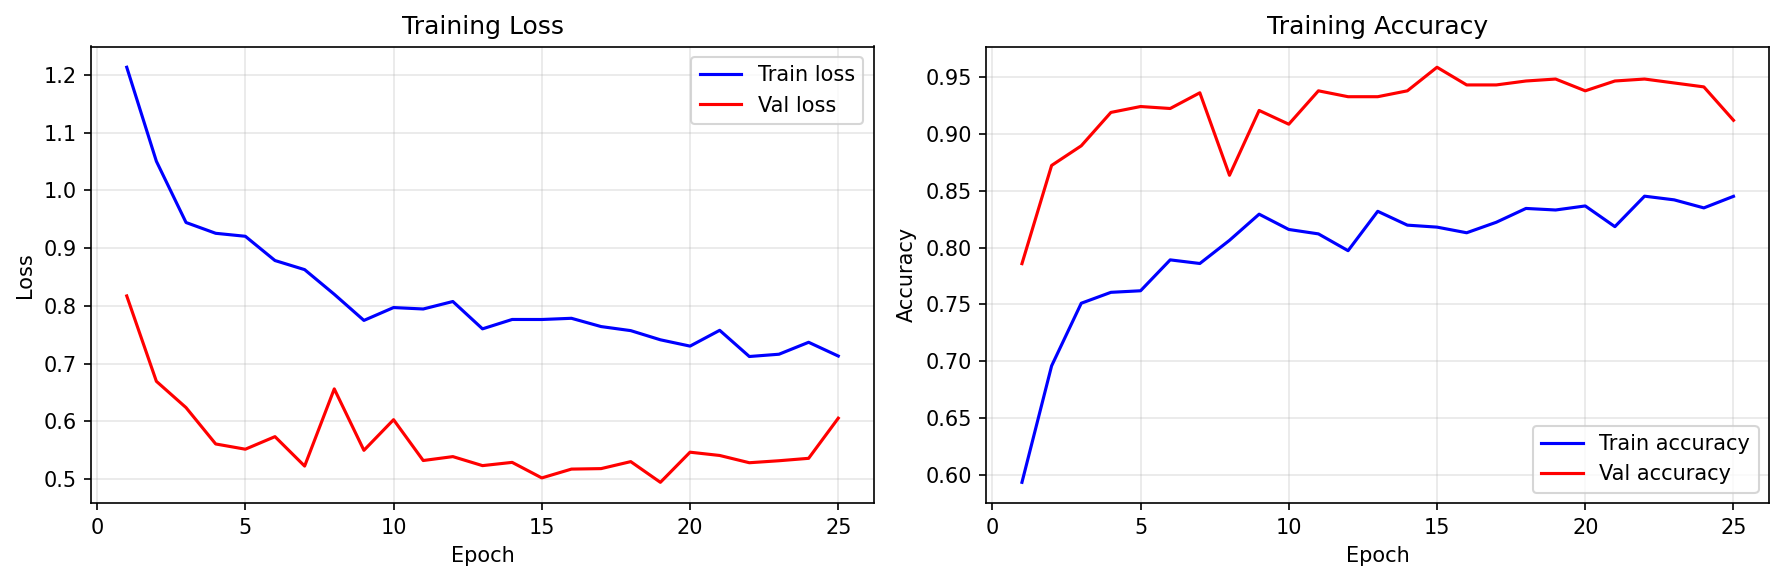
\includegraphics[width=\textwidth]{figures/hybrid_training_curves.png}
\caption{Кривые обучения гибридной модели: loss и accuracy для train и
validation выборок. Ось X - номер эпохи.}
\label{fig:training_curves}
\end{figure}

\section{Анализ ошибок}

Из 579 тестовых сэмплов модель ошиблась на 24 (4.1\%). Confusion matrix
(рис.~\ref{fig:confusion_hybrid}) показывает структуру ошибок.
Распределение ошибок по классам:
\begin{itemize}
    \item Superficial-Intermediate - 1/119 (0.8\%),
    \item Parabasal - 1/113 (0.9\%),
    \item Koilocytotic - \textbf{13/118 (11.0\%)} - основной источник
          ошибок,
    \item Dyskeratotic - 5/116 (4.3\%),
    \item Metaplastic - 4/113 (3.5\%).
\end{itemize}

Высокая доля ошибок на Koilocytotic ожидаема: койлоцитарные клетки
(ассоциированные с ВПЧ) морфологически близки к дискератоцитарным
(дисплазия) и метапластическим клеткам, все классы характеризуются
изменённой морфологией ядра. Это согласуется с известной сложностью
дифференциальной диагностики ВПЧ-инфекции и дисплазии в ручной цитологии
\cite{branca2015recommendations}.

\begin{figure}[H]
\centering
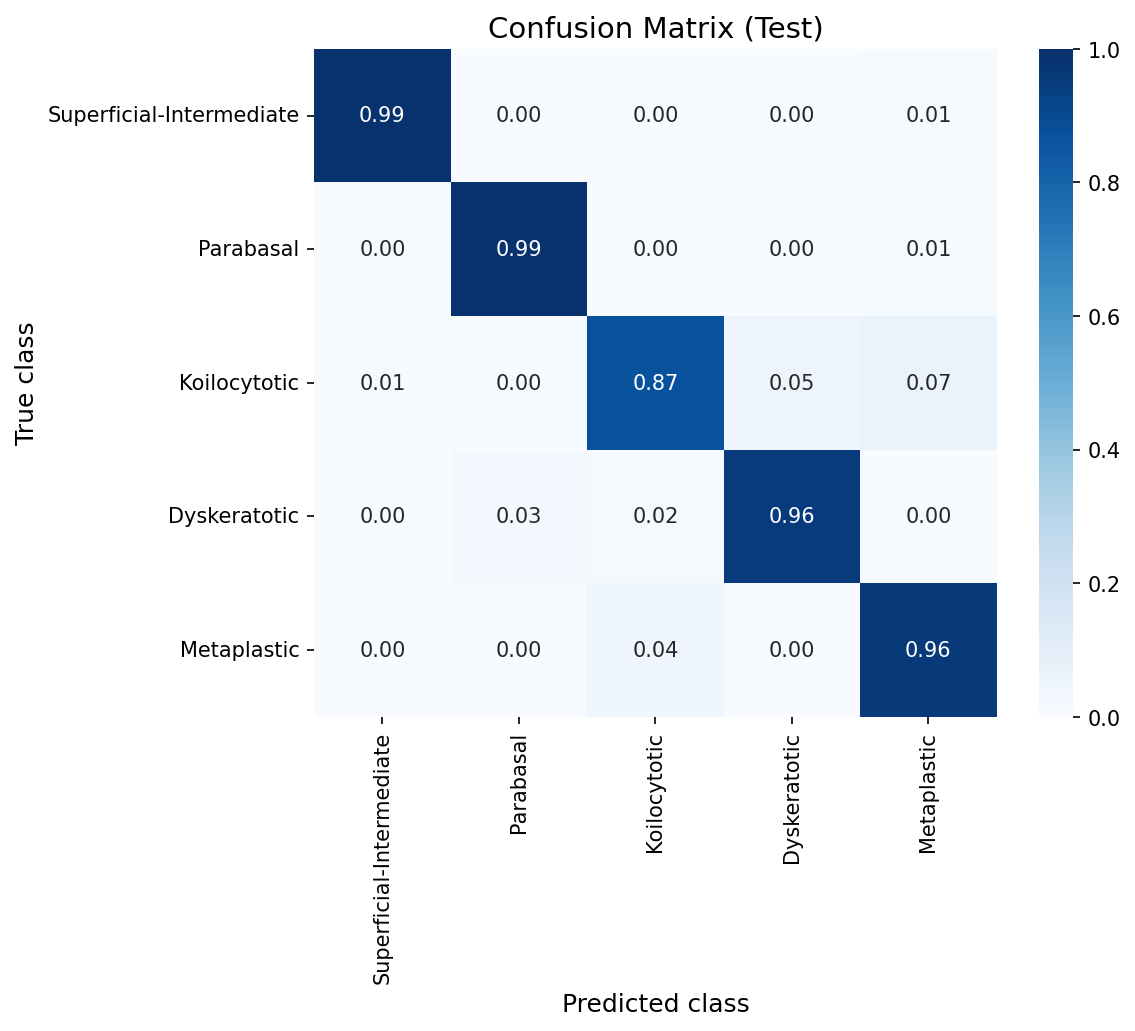
\includegraphics[width=0.85\textwidth]{figures/hybrid_confusion_matrix.png}
\caption{Confusion matrix HybridViTCNN на тестовой выборке (нормирована по
строкам). Основные потоки ошибок: Koilocytotic $\to$ Metaplastic (7\%),
Koilocytotic $\to$ Dyskeratotic (5\%), Metaplastic $\to$ Koilocytotic (4\%).}
\label{fig:confusion_hybrid}
\end{figure}

\begin{figure}[H]
\centering
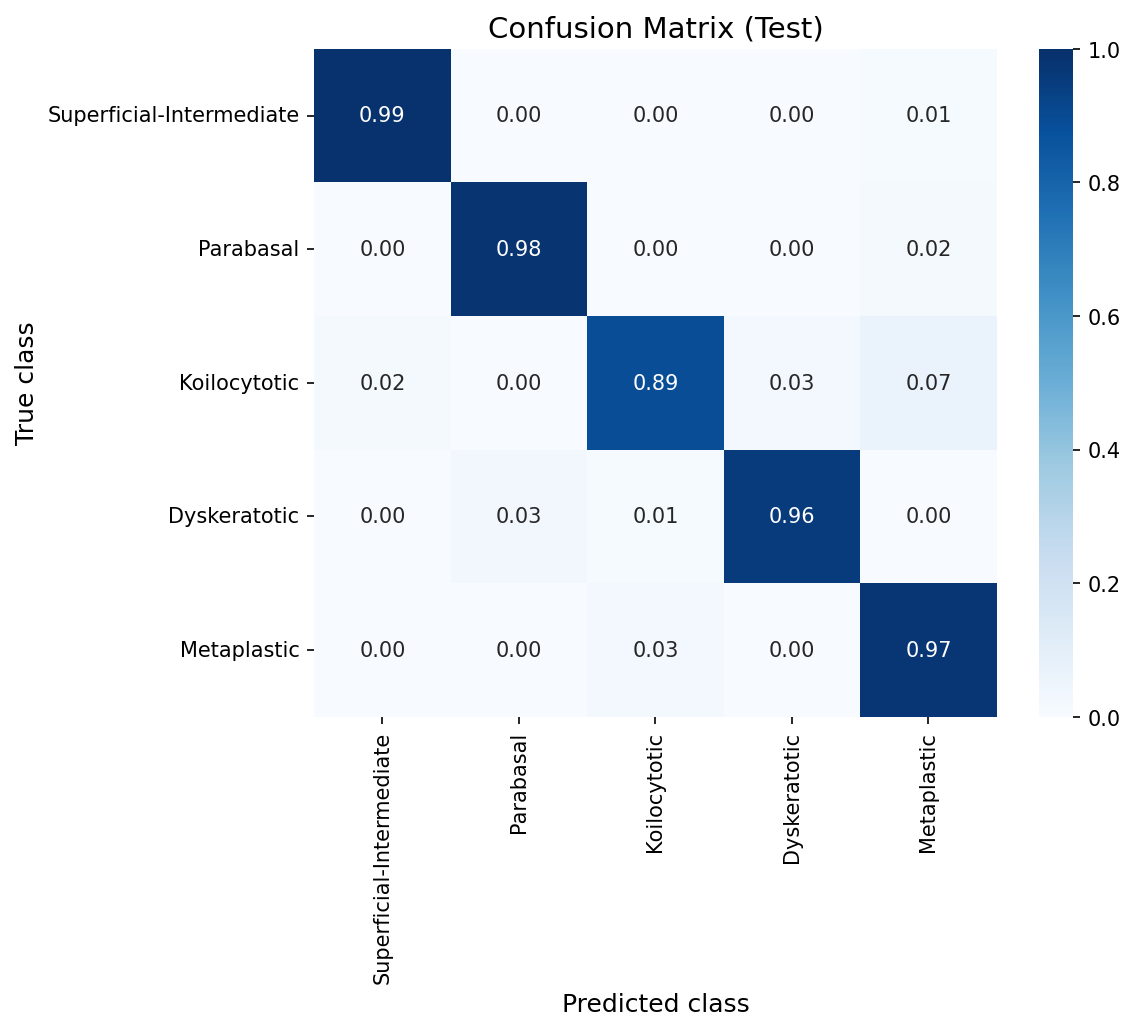
\includegraphics[width=0.85\textwidth]{figures/baseline_confusion_matrix.png}
\caption{Confusion matrix baseline-модели ConvNeXt-Base (без трансформера).
Структура ошибок аналогична гибриду: Koilocytotic - основной источник
путаниц, направление ошибок незначительно отличается
(Koilocytotic $\to$ Metaplastic 7\%, $\to$ Dyskeratotic 3\%,
$\to$ Superficial-Intermediate 2\%).}
\label{fig:confusion_baseline}
\end{figure}

Качественный анализ ошибочно классифицированных клеток представлен на
рис.~\ref{fig:wrong_predictions}: визуально многие из них действительно
близки к предсказанному классу - модель ошибается на пограничных
морфологиях, на которых ошибаются и цитологи.

\begin{figure}[H]
\centering
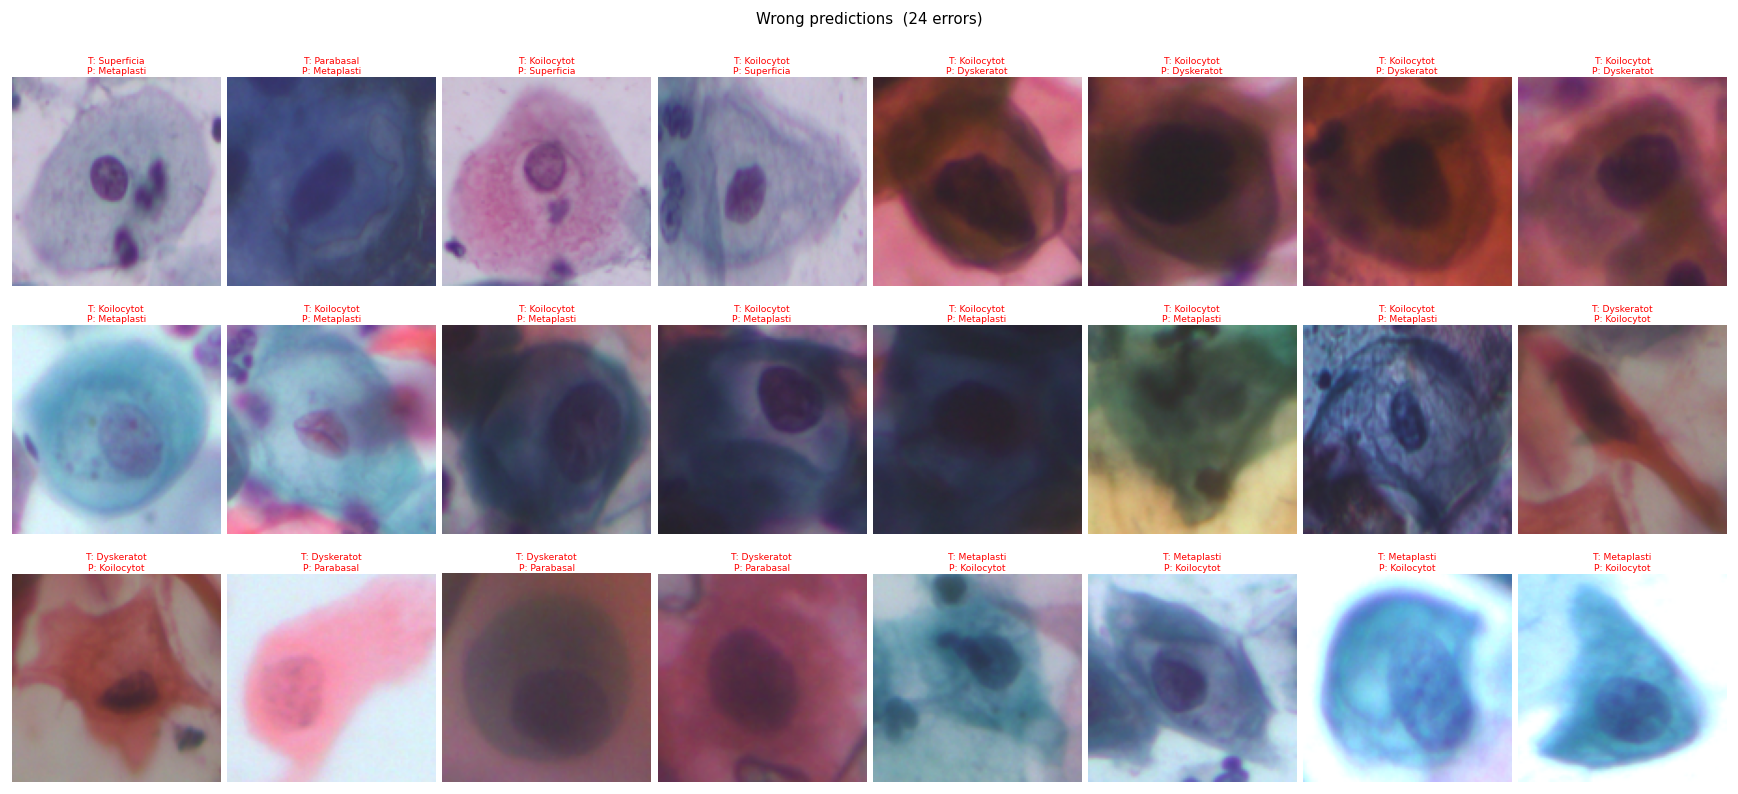
\includegraphics[width=\textwidth]{figures/wrong_predictions.png}
\caption{Примеры ошибочно классифицированных клеток (HybridViTCNN). Над
каждой клеткой: T - истинный класс, P - предсказанный класс.}
\label{fig:wrong_predictions}
\end{figure}

\section{Визуализация внимания}
\label{sec:attention}

Гибридная модель предоставляет метод \texttt{get\_attention\_maps()} для
извлечения весов self-attention из каждого трансформерного блока. Сырые веса
неинформативны без агрегации по слоям, поскольку каждый последующий блок
оперирует уже преобразованным представлением. Для получения интегральной
карты значимости применяется метод \textbf{attention rollout}
\cite{abnar2020rollout}.

\subsection{Attention rollout}

Пусть $A^{(l)} \in \mathbb{R}^{T \times T}$ - усреднённая по attention
heads матрица внимания на слое $l$ ($T = 50$ - 49 patch-токенов плюс CLS).
Для учёта residual-связей добавляется единичная матрица и строки
нормируются:
\[
    \tilde A^{(l)} = \mathrm{rownorm}\!\big(A^{(l)} + I\big).
\]
Итоговое внимание накапливается матричным произведением сверху вниз:
\[
    R^{(L)} = \tilde A^{(L)} \cdot \tilde A^{(L-1)} \cdots \tilde A^{(1)}.
\]
Карта значимости для CLS-токена - первая строка $R^{(L)}$ без диагонали:
$\mathbf{r}_{\mathrm{cls}} = R^{(L)}_{0, 1:} \in \mathbb{R}^{49}$. Этот
вектор переформируется в карту $7 \times 7$ и билинейно интерполируется до
исходного разрешения $224 \times 224$.

\subsection{Результаты}

Реализация - CLI-команда \texttt{lunicyto attention --checkpoint <path>},
которая загружает лучший чекпойнт, прогоняет несколько сэмплов из тестовой
выборки и сохраняет grid с оригиналами и наложенными heatmap
(рис.~\ref{fig:attention_maps}).

\begin{figure}[H]
\centering
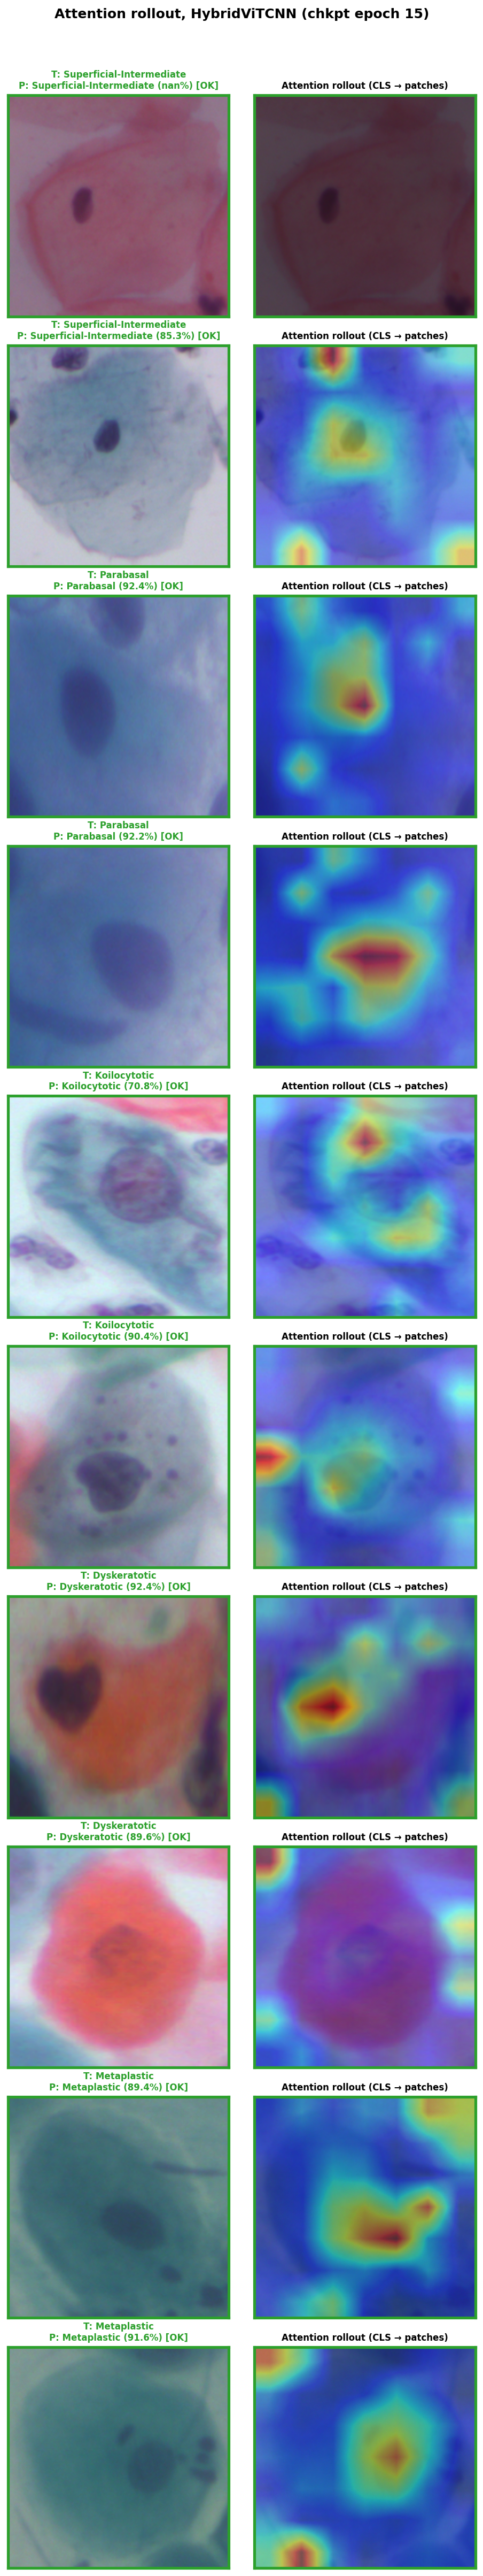
\includegraphics[width=\textwidth,height=0.70\textheight,keepaspectratio]{figures/attention_maps.png}
\caption{Attention rollout для гибридной модели на тестовых сэмплах
(2 примера на класс, 10 изображений всего). Слева - оригинал, справа -
наложение карты внимания CLS $\to$ patches. Зелёная рамка -
верно классифицировано, красная - ошибочно. Над каждым изображением:
T - истинный класс, P - предсказание с confidence в \%.
Карты внимания концентрируются на ядре клетки и перинуклеарной области,
что соответствует биологически значимым признакам цитологической
классификации (размер и форма ядра, ядерно-цитоплазматическое
соотношение, наличие гало).}
\label{fig:attention_maps}
\end{figure}

Baseline-модель такой возможности из коробки не предоставляет - в ней
global-average-pooling сжимает пространственную информацию до вектора, и
визуализация фокуса требует внешних методов (Grad-CAM), не присущих
архитектуре. Это один из практических преимуществ гибрида для медицинских
CAD-сценариев, где интерпретируемость решения требуется регуляторно.

\chapter{Программная реализация}
\label{ch:impl}

\section{Структура пакета}

Программная часть работы оформлена в виде установочного Python-пакета
\texttt{lunicyto}, размещённого в репозитории проекта. Структура:

\begin{lstlisting}[basicstyle=\ttfamily\footnotesize]
lunicyto/
  config/
    train.toml
    train_baseline.toml
  src/lunicyto/
    cli.py
    datasets/sipakmed.py
    models/
      hybrid_vit_cnn.py
      baseline.py
    training/
      trainer.py
      metrics.py
      early_stopping.py
    utils/
      train.py
      cross_validate.py
      attention_viz.py
      download_data.py
      explore.py
      models.py
  thesis/
    main.tex
    figures/
  pyproject.toml
\end{lstlisting}

Каждая функция CLI принимает путь к TOML-конфигу и опционально
override-параметры. TOML выбран как формат конфигурации: он строго
типизирован, поддерживается стандартной библиотекой Python 3.11+
(\texttt{tomllib}), и в отличие от YAML не имеет двусмысленностей с
булями и числами с плавающей точкой.

\section{Команды CLI}

\begin{itemize}
    \item \texttt{lunicyto info --data-dir <path>} - быстрая проверка
          датасета: количество изображений по классам, пример
          изображения, классовое распределение.
    \item \texttt{lunicyto download} - скачивание SIPaKMeD с Kaggle
          (требует валидных credentials в \texttt{\~/.kaggle/}).
    \item \texttt{lunicyto train --config <toml>} - обучение по
          конфигу. Создаёт уникальный по timestamp подкаталог в
          \texttt{output.dir}, сохраняет туда чекпойнт, отчёт,
          картинки, копию конфига.
    \item \texttt{lunicyto cv --config <toml> --folds K} - $K$-fold
          стратифицированная group-aware кросс-валидация. Каждый фолд
          получает собственный подкаталог \texttt{fold\_i/}, общая
          сводка пишется в \texttt{cv\_summary.txt}.
    \item \texttt{lunicyto attention --checkpoint <pth> --config <toml>}
          - генерация attention-rollout grid из лучшего чекпойнта
          гибрида.
\end{itemize}

Все команды используют единый Typer-app, описание видно через
\texttt{lunicyto --help}.

\section{Валидация конфигурации}

Все TOML-конфиги валидируются Pydantic-моделями
(\texttt{utils/models.py}): размеры, диапазоны float, ограничения на
строки. При попытке передать невалидный конфиг (например, batch\_size
$< 1$ или drop\_path\_rate $> 1$) приложение падает на старте с
информативным сообщением, до загрузки данных и модели. Это экономит
время на длинных прогонах.

\section{Метрики и логирование}

Метрики собираются по batch'ам и агрегируются после прохода через всю
валидационную/тестовую выборку. На обучении в каждой эпохе пишутся в
TensorBoard: train/val loss, train/val accuracy, F1 macro, AUC macro,
текущий learning rate (для head-группы параметров). Это позволяет
параллельно следить за несколькими прогонами, не сравнивая текстовые
логи. Финальная оценка на тесте проводится с
\textbf{test-time augmentation} (TTA): для каждого батча предсказание
усредняется по четырём флипам - оригинал, флип по горизонтали, флип
по вертикали, флип по обеим осям. Реализация - в
\texttt{Trainer.\_evaluate}.

\section{Воспроизведение результатов}

Минимальный шаг для воспроизведения основного результата:

\begin{lstlisting}[basicstyle=\ttfamily\footnotesize]
uv tool install --editable lunicyto@.

lunicyto download

lunicyto info --data-dir data/sipakmed

export PYTORCH_CUDA_ALLOC_CONF=expandable_segments:True
lunicyto train --config config/train.toml

lunicyto train --config config/train_baseline.toml

lunicyto cv --config config/train.toml --folds 5

lunicyto attention \
    --checkpoint runs/experiment_001/<ts>/best_model.pth \
    --config config/train.toml
\end{lstlisting}

На указанной конфигурации (RTX 2060 6\,GB) один полный прогон
гибридной модели занимает примерно 25--30 минут, baseline -
20--25 минут, 5-fold CV - около 2--2.5 часов.

\chapter*{Заключение}
\addcontentsline{toc}{chapter}{Заключение}
\label{ch:conclusion}

В работе разработана и оценена гибридная нейросетевая модель для
многоклассовой классификации клеток в цитоскрининге - комбинация
ConvNeXt-Base в роли извлекателя локальных признаков и Vision-Transformer
энкодера в роли агрегатора глобального контекста. Помимо архитектурного
вклада, выполнен ряд методических улучшений по сравнению с типичной для
литературы практикой работы с SIPaKMeD: явная защита от утечки между
слайдами, аблационное сравнение, кросс-валидация, визуализация внимания и
полностью воспроизводимый пайплайн в виде установочного Python-пакета.

Основные результаты:

\begin{enumerate}
    \item Выявлена и исправлена типичная ошибка пайплайна загрузки данных
          SIPaKMeD: вложенная структура архива (\texttt{im\_X/im\_X/CROPPED/})
          при использовании \texttt{os.listdir()} или \texttt{Path.iterdir()}
          без рекурсии приводит к нулевой обучающей выборке. В работе пайплайн
          явно адресует подкаталог \texttt{CROPPED/} каждого класса.
    \item Реализована гибридная модель HybridViTCNN на базе ConvNeXt и
          Transformer encoder с улучшенными техниками обучения (label
          smoothing, Mixup, RandAugment, stochastic depth, раздельные LR).
    \item Применено стратифицированное разбиение датасета, обеспечивающее
          корректную оценку обобщающей способности модели.
    \item Модель достигает на тестовой выборке Accuracy 95.51\%,
          F1 macro 95.48\%, AUC-ROC macro 99.72\% - результат
          конкурентоспособен с современными single-model подходами и
          получен с явной защитой от утечки слайдов.
    \item Проведено аблационное сравнение с baseline (ConvNeXt-Base без
          трансформерного энкодера): top-1 метрики обеих моделей лежат в
          пределах статистической дисперсии одного сплита, однако гибрид
          даёт более калиброванные вероятностные выходы (AUC +0.39 п.п.)
          и предоставляет attention-карты для интерпретации решения -
          свойства, важные для применения в CAD-системах.
    \item Проведена 5-fold кросс-валидация со стратификацией и
          группировкой по слайду: Accuracy $94.42 \pm 1.42$\%,
          F1 $94.41 \pm 1.43$\%, AUC $99.04 \pm 0.95$\%. Дисперсия по
          фолдам подтверждает корректность оценки и количественно
          определяет статистическую неопределённость результата.
\end{enumerate}

\section{Ограничения}

Ряд ограничений работы заслуживает явного упоминания.

\textbf{Один центр сбора данных.} SIPaKMeD собран в одном медицинском
учреждении при одинаковом протоколе окрашивания и одинаковом оборудовании
для оцифровки. Обобщение модели на изображения, полученные на другом
оборудовании или с другим протоколом окрашивания (например, LBC vs
традиционный мазок), не проверено и без отдельного тестирования
гарантировано быть не может. Это типичная проблема медицинского DL,
известная как domain shift. Решение - внешняя валидация на независимом
датасете (например, Herlev) и/или domain-adaptation подходы.

\textbf{Размер датасета.} 4049 изображений - сравнительно малый объём
для глубокой архитектуры в 117M параметров. Прогресс над baseline 89M
параметров оказался скромным; есть основания полагать, что
трансформерная часть здесь работает на пределе своих возможностей и
дополнительные данные дали бы больший выигрыш именно гибриду, тогда как
у CNN-baseline точность ближе к насыщению.

\textbf{Дисперсия оценки.} CV показала $\sigma = 1.4$\% по accuracy,
причём фолд 3 заметно «провалился» (91.98\% vs 96.17\% для фолда 5).
Это говорит о существенной зависимости от состава тестового сплита:
если все «трудные» слайды собраны в один фолд, точность модели падает.
Для клинического применения это означает, что числа из любой одиночной
оценки следует интерпретировать с поправкой на $\pm 2$ п.п.

\textbf{Только классификация изолированных клеток.} Реальный
скрининговый сценарий включает два этапа: сегментация/детекция клеток
на широком поле зрения, затем классификация. В данной работе решается
только второй этап (исходные кропы SIPaKMeD уже выделены). Интеграция в
сквозной пайплайн остаётся отдельной инженерной задачей.

\textbf{Отсутствие клинической валидации.} Модель оценена по техническим
метрикам (Acc, F1, AUC). Клиническая ценность определяется иными
показателями (PPV, NPV в популяции с известной prevalence, time-to-result,
влияние на принятие решения врачом). Подобные испытания выходят за рамки
дипломной работы.

\section{Направления дальнейших исследований}

\begin{itemize}
    \item \textbf{Внешняя валидация.} Прогон обученной модели на
          датасете Herlev и/или собственных данных для оценки
          domain-generalisation.
    \item \textbf{Поднятие точности на Koilocytotic.} Этот класс
          остаётся слабым звеном (recall $\approx 0.87$). Возможные
          подходы: class-balanced sampler, focal loss, целевая
          аугментация (CutMix), отдельное pre-training на ВПЧ-датасете.
    \item \textbf{Whole-slide images (WSI).} Адаптация к большим полям
          зрения через схему «детекция + классификация», возможно с
          использованием результатов \cite{zhang2025large}.
    \item \textbf{Дистилляция и квантование.} Уменьшение модели для
          edge-инференса в полевых условиях, особенно для регионов с
          ограниченной инфраструктурой.
    \item \textbf{Калибровка и неопределённость.} Применение
          temperature scaling, Monte Carlo dropout или deep ensembles
          для получения честных оценок неопределённости - критично
          для медицинского принятия решений.
    \item \textbf{Объединение с биомаркерами.} Совместное использование
          цитоморфологии и анализа ВПЧ-ДНК (Hybrid Capture, PCR) для
          повышения PPV скрининговой схемы.
\end{itemize}

\renewcommand{\bibname}{Список литературы}
\begin{thebibliography}{99}
\addcontentsline{toc}{chapter}{Список литературы}

\bibitem{bray2018global}
Bray~F. et~al. Global cancer statistics 2018: GLOBOCAN estimates of
incidence and mortality worldwide for 36 cancers in 185 countries~//
CA: A Cancer Journal for Clinicians. 2018. Vol.~68. P.~394--424.

\bibitem{curry2018screening}
Curry~S.J. et~al. Screening for Cervical Cancer: US Preventive Services
Task Force Recommendation Statement~// JAMA. 2018. Vol.~320. P.~674--686.

\bibitem{hashmi2020comparison}
Hashmi~A.A. et~al. Comparison of Liquid-Based Cytology and Conventional
Papanicolaou Smear for Cervical Cancer Screening~// Cureus. 2020.
Vol.~12. Art.~e12293.

\bibitem{branca2015recommendations}
Branca~M., Longatto-Filho~A. Recommendations on Quality Control and
Quality Assurance in Cervical Cytology~// Acta Cytologica. 2015.
Vol.~59. P.~361--369.

\bibitem{lecun2015deep}
LeCun~Y., Bengio~Y., Hinton~G. Deep learning~// Nature. 2015. Vol.~521.
P.~436--444.

\bibitem{zhang2025large}
Zhang~X. et~al. A large annotated cervical cytology images dataset for
AI models to aid cervical cancer screening~// Scientific Data. 2025.
Vol.~12. Art.~23.

\bibitem{cervigan2025}
Karadag~A. et~al. CerviGAN: Cervical cancer pap smear image classification
with GAN-based data augmentation and external attention transformer~//
Applied Intelligence. Springer, 2025.

\bibitem{li2019detection}
Li~X., Li~Q. Detection and classification of cervical exfoliated cells
based on faster R-CNN~// IEEE ICAIT. 2019. P.~52--57.

\bibitem{xiang2020novel}
Xiang~Y. et~al. A novel automation-assisted cervical cancer reading method
based on convolutional neural network~// Biocybernetics and Biomedical
Engineering. 2020. Vol.~40. P.~611--623.

\bibitem{ma2020macd}
Ma~B. et~al. MACD R-CNN: an abnormal cell nucleus detection method~//
IEEE Access. 2020. Vol.~8. P.~166658--166669.

\bibitem{randel2013acog}
Randel~A. ACOG Releases Guideline on Cervical Cancer Screening~//
American Family Physician. 2013. Vol.~88. P.~776--777.

\bibitem{plissiti2018sipakmed}
Plissiti~M.E. et~al. SIPaKMeD: A New Dataset for Feature and Image Based
Classification of Normal and Pathological Cervical Cells in Pap Smear
Images~// ICIP. 2018. P.~3144--3148.

\bibitem{cerviformer2023}
Baid~U. et~al. CerviFormer: A Pap-smear based cervical cancer classification
method using cross attention and latent transformer~// arXiv:2303.10222. 2023.

\bibitem{hybridvit2025}
Al-Dabet~M.M. et~al. A hybrid vision transformer with ensemble CNN framework
for cervical cancer diagnosis~// BMC Medical Informatics and Decision Making.
2025. Vol.~25. Art.~152.

\bibitem{liu2022convnext}
Liu~Z. et~al. A ConvNet for the 2020s~// IEEE/CVF CVPR. 2022. P.~11976--11986.

\bibitem{cubuk2020randaugment}
Cubuk~E.D. et~al. RandAugment: Practical automated data augmentation with a
reduced search space~// NeurIPS. 2020. Vol.~33. P.~18613--18624.

\bibitem{zhang2018mixup}
Zhang~H. et~al. Mixup: Beyond empirical risk minimization~// ICLR. 2018.

\bibitem{huang2016deep}
Huang~G. et~al. Deep networks with stochastic depth~// ECCV. 2016.
P.~646--661.

\bibitem{abnar2020rollout}
Abnar~S., Zuidema~W. Quantifying Attention Flow in Transformers~//
Proceedings of the 58th Annual Meeting of the Association for
Computational Linguistics (ACL). 2020. P.~4190--4197.

\bibitem{kaggle_sipakmed}
Cervical Cancer largest dataset (SipakMed). Kaggle.
\url{https://www.kaggle.com/datasets/prahladmehandiratta/cervical-cancer-largest-dataset-sipakmed}

\end{thebibliography}

\end{document}
